\chapter{State of The Art}
\section{Virtual Counters}
Virtual Counters, or Guichets Virtuels in French, are online platforms that allow users to access services remotely without having to physically visit a location. They are designed to facilitate the interaction between users and service providers in a user-friendly, efficient and secure manner. The rise of digital technology has led to the development of various types of virtual counters, each with its own features and benefits.

\subsection{Types of Virtual Counters}
There are various types of virtual counters, such as:
\begin{itemize}
    \item \textbf{Web-based virtual counters:} These virtual counters are accessible through a web browser, and they allow users to access various online services offered by service providers.
    \item \textbf{Mobile-based virtual counters:} These virtual counters are accessible through mobile devices such as smart-phones and tablets, and they offer users the convenience of accessing services on the go.
    \item \textbf{Kiosk-based virtual counters:} These virtual counters are installed in designated locations and allow users to access various services through self-service kiosks.
    \item \textbf{Chat-based virtual counters:} These virtual counters use instant messaging applications to facilitate communication between users and service providers, allowing users to access services through a chat-bot or live chat.
\end{itemize}

\subsection{Examples of Virtual Counters}
Virtual counters have become increasingly popular in Algeria, and several organizations have adopted them to improve their services. Some examples of virtual counters in Algeria include:

\begin{itemize}
  \item \textbf{ElHanna:} The Caisse Nationale de l'Assurance Maladie (CNAS) in Algeria has created an application called "El Hanna" that allows its members to access various services related to their health insurance coverage, such as checking their eligibility for medical procedures, viewing their medical history
  \item \textbf{BaridiMob:} Algérie Poste has developed a virtual counter that allows customers to access their banking services online, such as transferring funds and paying bills.
  \item \textbf{Sonelgaz:} Sonelgaz has developed a virtual counter that allows customers to access their energy bills and make payments online.
  \item \textbf{Algerie Telecom E-Paiement:} Algerie Telecom E-Paiement is a mobile application-based electronic payment service provided by Algerie Telecom. It offers customers a secure and convenient platform to make online payments, pay bills, recharge mobile credit, and make purchases using their smartphones. By embracing mobile technology, Algerie Telecom E-Paiement enhances the accessibility and convenience of electronic payments in Algeria.\cite{elhanna-source}
\end{itemize}

Virtual counters have also been implemented in other countries, such as:

\begin{itemize}
  \item \textbf{eVisa:} The eVisa platform allows travelers to apply for visas online, reducing the need to physically visit an embassy or consulate.
  \item \textbf{eCNI:} The eCNI platform in France allows citizens to apply for their national identity cards online, reducing the need to visit a physical office.
\end{itemize}

In the next section, we will explore the benefits of virtual counters and their impact on the user experience.

\subsection{Benefits of Virtual Counters}
Virtual counters offer several benefits for both users and service providers. Some of the key benefits include:

\begin{itemize}
    
\item \textbf{Convenience:}  Virtual counters can be accessed from anywhere with an internet connection, making it more convenient for people to access services without having to physically go to a government office.
\item \textbf{Time-saving:} Virtual counters eliminate the need for users to physically visit a service center, saving them time and effort. Users can complete their transactions from the comfort of their own homes or offices, without having to wait in long lines or take time off work.
\item \textbf{Accessibility:} Virtual counters provide users with greater accessibility to services. They can access services from anywhere, at any time, as long as they have an internet connection. This is particularly beneficial for people with disabilities or those who live in remote areas and have limited access to physical service centers.
\item \textbf{Efficiency:} Virtual counters streamline the service delivery process by reducing paperwork, eliminating redundancies, and increasing transparency. This allows service providers to process transactions more efficiently and with greater accuracy.
\item \textbf{Cost-effective:} Virtual counters are typically more cost-effective for service providers than physical service centers. They require less physical infrastructure, fewer staff, and have lower operating costs. This can help service providers reduce costs and improve their bottom line.
\end{itemize}

\subsection{Challenges and Limitations}

Despite the benefits of virtual counters, there are also some challenges and limitations to consider. These include:
\begin{itemize}
    \item \textbf{Access and Connectivity}

One of the biggest challenges of virtual counters is ensuring that they are accessible to everyone, regardless of their location or technical ability. This requires reliable internet connectivity, as well as user-friendly interfaces and support for multiple languages.
\item \textbf{Security and Privacy}

Virtual counters also raise concerns about security and privacy. Users may be hesitant to share sensitive personal information online, and there is always the risk of data breaches or cyber attacks.
\item \textbf{Digital Divide}

Another limitation of virtual counters is the digital divide, which refers to the gap between those who have access to digital technologies and those who do not. This can be a particular challenge in developing countries or among low-income populations.
\item \textbf{Technical Issues}

Finally, virtual counters may also face technical issues such as server downtime, software bugs, or compatibility problems with different devices and platforms. These can all affect the user experience and the efficiency of the service.
\end{itemize}
Despite these challenges, virtual counters have the potential to revolutionize the way we access public services and interact with government agencies. By addressing these limitations, we can ensure that virtual counters are accessible, secure, and efficient for everyone.

\section{Introduction to CNAS Organization}
\subsection{Definition of CNAS organization}
The CNAS (Caisse Nationale des Assurances Sociales) is a public institution with specific management under Article 49 of Law No. 88-01 of January 12, 1988. It has legal personality and financial autonomy and is considered a merchant in its relations with third parties. The CNAS is responsible for managing social insurance benefits (illness, maternity, disability, and death), as well as occupational accidents and diseases (AO/D), and family allowances on behalf of the state. It also manages the collection, control, and litigation of contributions for financing benefits, as well as the management of the litigation related to the collection of subscriptions for financing rendered.

The CNAS assigns a national registration number to insured persons and employers and contributes to promoting the policy of prevention of AO/D and managing the AO/D prevention fund. It also manages benefits for beneficiaries of bilateral social security agreements, carries out medical control of beneficiaries, and undertakes actions to provide workers and their dependents with collective benefits in the form of health and social achievements. The CNAS also manages the aid and relief fund and concludes agreements with healthcare providers while ensuring the information of beneficiaries and employers.

The CNAS provides benefits to salaried workers, apprentices, job seekers, students, trainees in vocational training, disabled persons, veterans, social security beneficiaries (pensioners and annuitants), and beneficiaries of the lump sum solidarity allowance (sick, elderly and inactive persons). Dependents, including the spouse, minor children, unmarried inactive daughters, and dependent ascendants, are also eligible for benefits.

The CNAS covers healthcare and medication costs at 80\%, and in some cases 100\% (particularly for chronic diseases). Compensation for sick leave is 50\% of the salary for the first 15 days and is increased to 100\% of the salary beyond the 16th day, with a maximum duration of three years. Maternity benefits are fully covered, and working women are entitled to a 98-day maternity leave. The minimum amount of invalidity pensions is equal to 75\% of the guaranteed minimum wage. In the event of the insured person's death, a death benefit is paid to his or her dependents. Occupational risks are covered 100\% for healthcare and sick leave, and annuities are paid in the event of bodily harm or death resulting from occupational accidents or diseases.
\cite{cnas-presentation}
\subsection{Organization of CNAS}
CNAS is managed by a Board of Directors and is under the supervision of the Minister of Labor, Employment and Social Security. Its headquarters is located in Algiers (BEN AKNOUN), and it has national jurisdiction with both central and local services.\footnote{CNAS. (n.d.). Presentation of CNAS. Retrieved from \url{https://www.cnas.dz/}.}

\medskip To fulfill its missions, CNAS has: 
\begin{table}[htbp]
  \centering
  \begin{tabular}{|p{10cm}|l|}
  \hline
  \textbf{Structure} & \textbf{Number} \\
  \hline
  General Directorate & 1 \\
  \hline
  Provincial agencies(including 2 in Algiers)  & 49 \\
  \hline
  Payment structures & 826 \\
  \hline
  Payment centers & 356 \\
  \hline
  Payment branches & 401 \\
  \hline
  Local correspondences & 69 \\
  \hline
  Specialized clinics (pediatric heart surgery, orthopedics and rehabilitation, ENT, dental) & 4 \\
  \hline
  Regionval centers for medical imaging & 4 \\
  \hline
  Diagnostic and treatment centers & 35 \\
  \hline
  Pharmaceutical offices & 55 \\
  \hline
  Nurseries and kindergartens & 30 \\
  \hline
  Printing house in Constantine & 1 \\
  \hline
  Family social center in Ben Aknoun & 1 \\
  \hline
  \end{tabular}
  \caption{CNAS Structures}
  \end{table}

\newpage
\subsection{CNAS Organigram}
the CNAS organigram is made up of various departments, subdivisions, and services that work together to manage CNAS operations and deliver services to its beneficiaries.\cite{organigram-source}


\medskip

Here is the CNAS organigram : 
\begin{figure}[h]
  \centering
  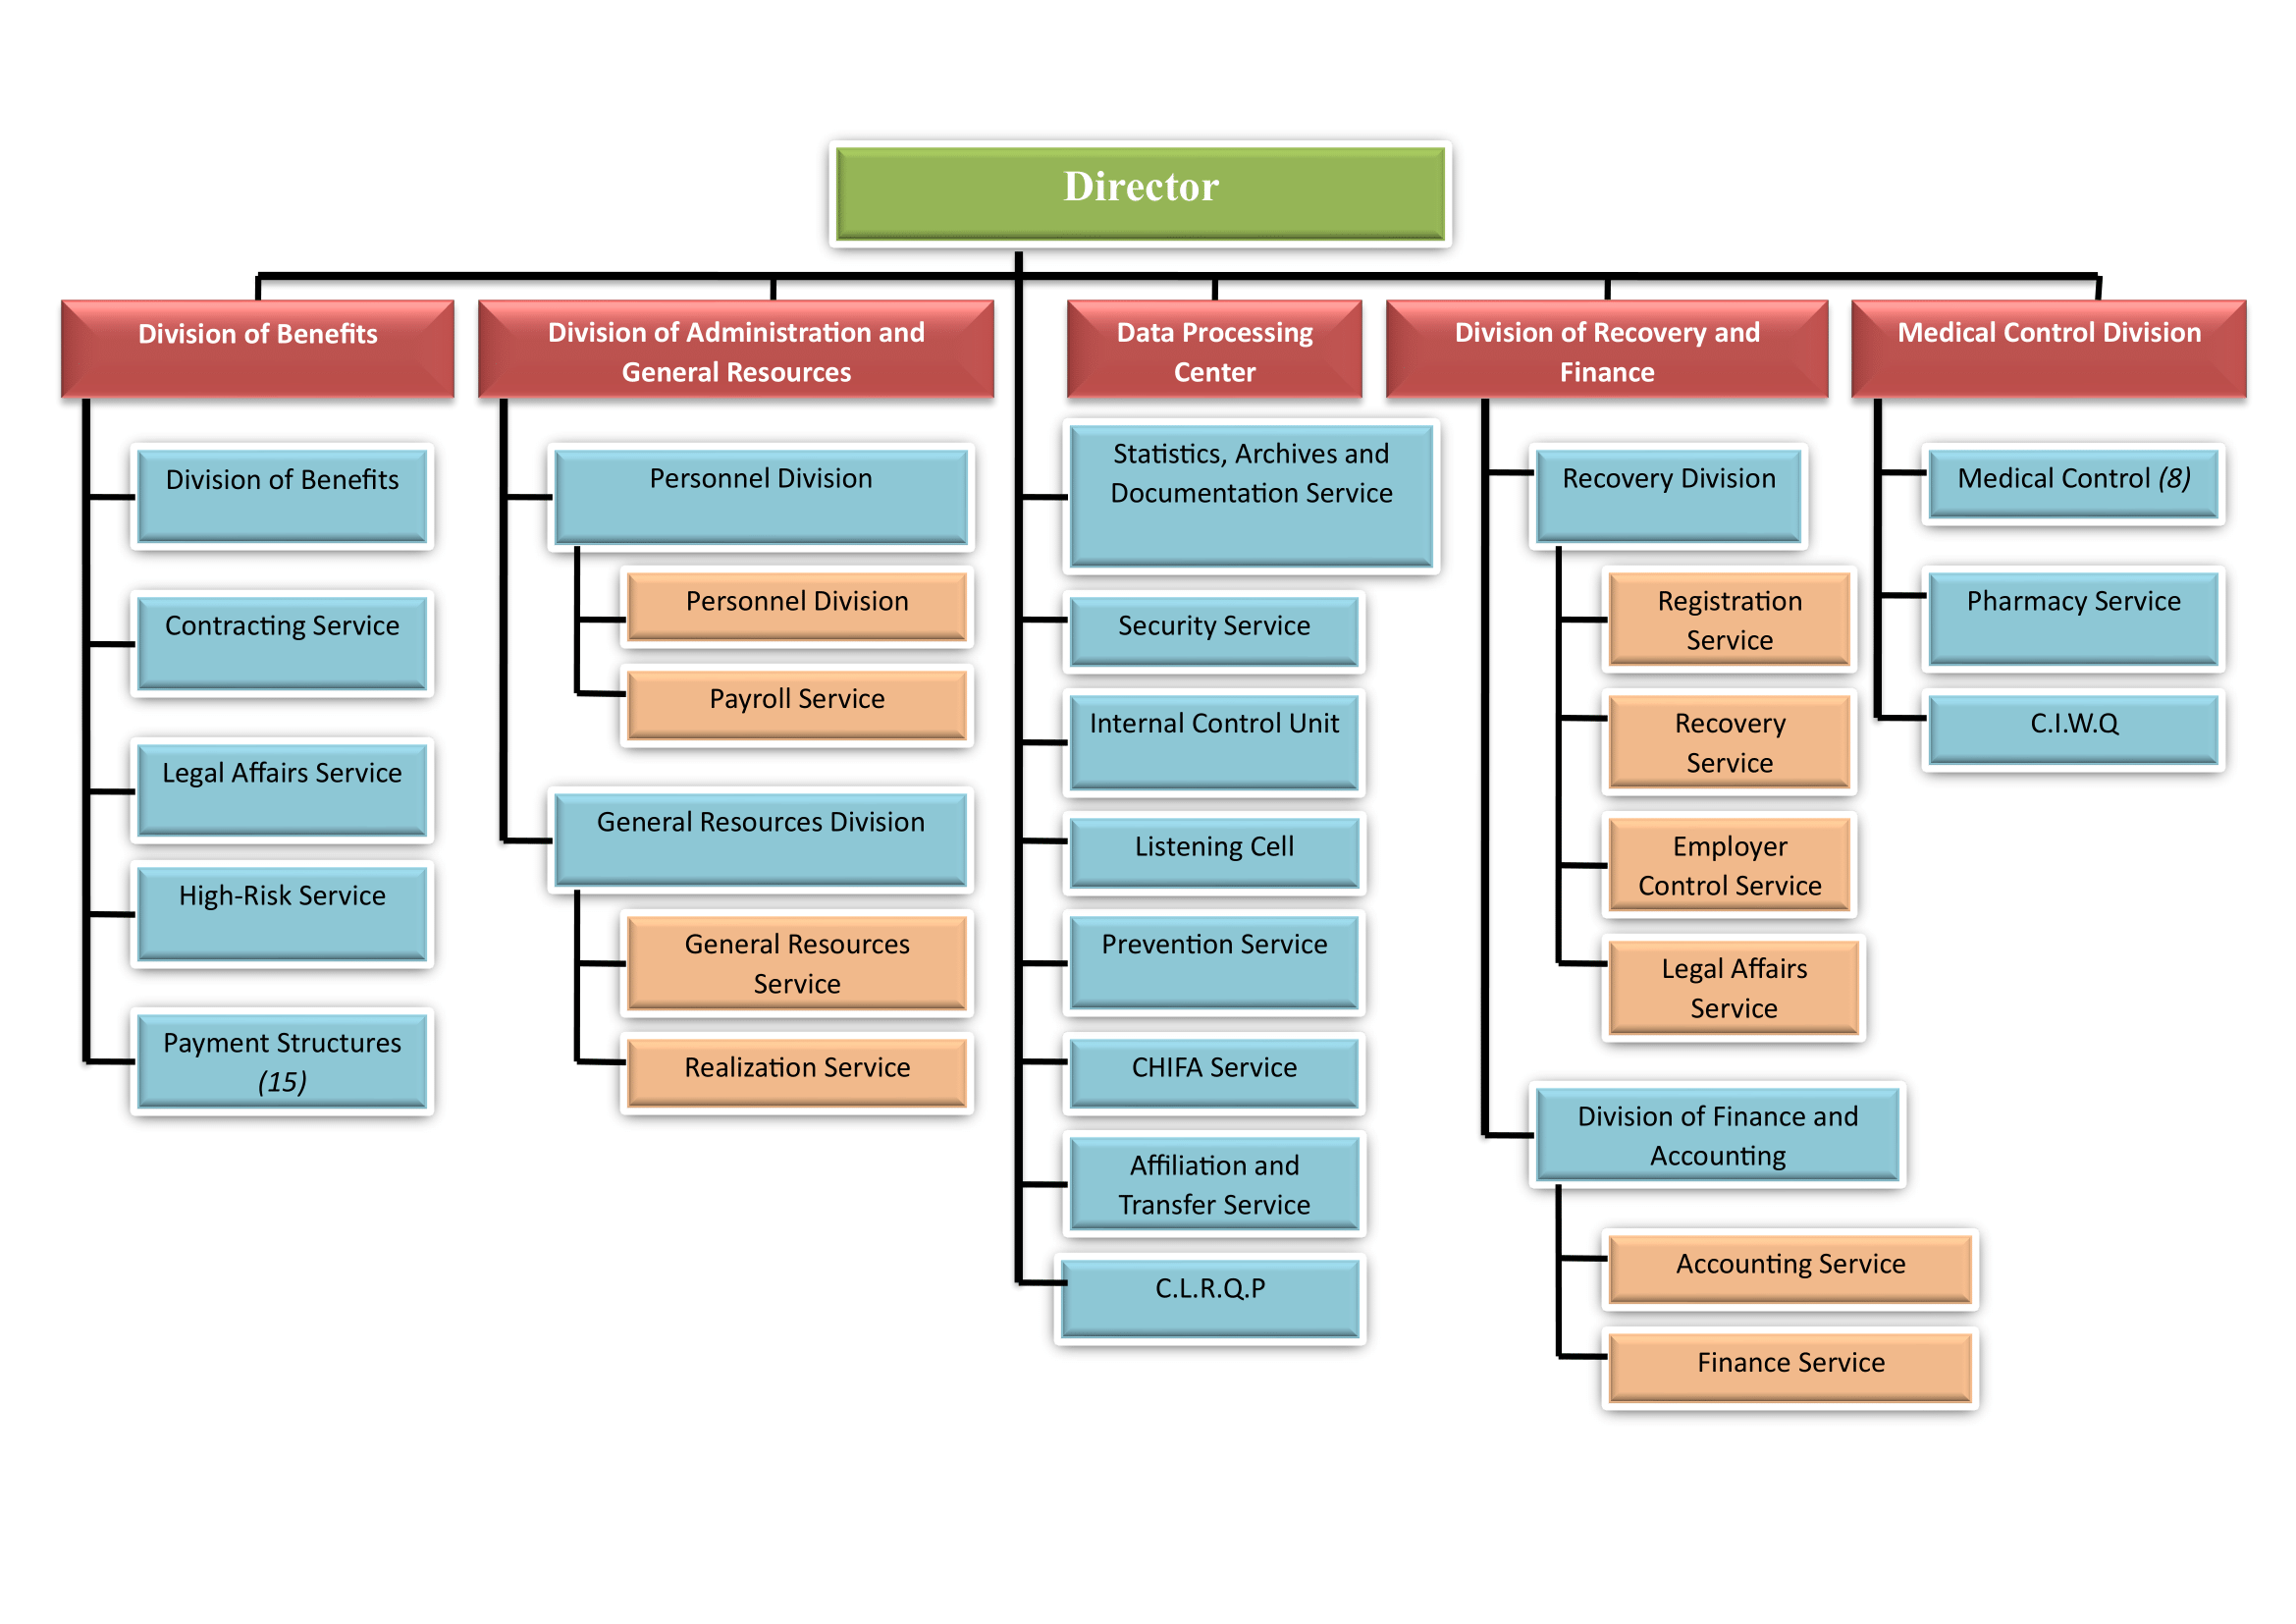
\includegraphics[width=1.0\textwidth]{cnas organigramme-1.png}
  \caption{Organigram of CNAS}
  \label{fig:organigram}
\end{figure}
\subsection{CNAS Services}
CNAS provides a range of services related to social security and healthcare to the Algerian population. These services include:
\begin{itemize}
    \item \textbf{Healthcare services:} CNAS operates its own specialized clinics and medical facilities, including four specialized clinics for cardiac surgery, orthopedics and rehabilitation, otorhinolaryngology, and dental care. It also runs 35 diagnostic and treatment centers, 55 pharmacies, and four regional medical imaging centers.

    \item \textbf{Social security services:} CNAS provides social security services to its members and their families, including health insurance, maternity leave benefits, disability benefits, and retirement pensions. It also offers services related to workplace safety and injury compensation.

    \item \textbf{Family services:} CNAS operates 30 nurseries and childcare centers to support working parents.

    \item \textbf{Payment services:} CNAS manages a network of payment centers and local correspondents to ensure the timely payment of social security benefits to its members.
\end{itemize}
\subsection{  Importance of CNAS services for the Algerian society}
These services are essential for the Algerian society, as they help provide access to healthcare and social security benefits to millions of people. CNAS's role in ensuring workplace safety and providing compensation for work-related injuries is also crucial in protecting the rights and wellbeing of workers across Algeria.

\section{Literature Review}
\label{sec:literature-review}

Virtual counters and appointment management systems have emerged as essential tools in various domains, revolutionizing the way organizations handle customer interactions and streamline service processes. In this literature review, we explore the significance of virtual counters, and we discuss the importance of adopting web-based solutions for appointment management, highlighting the benefits they offer to CNAS and similar organizations.

Virtual counters provide an innovative approach to managing customer queues and optimizing service delivery. They enable users to access services remotely, eliminating the need for physical presence and reducing waiting times. CNAS's El Hanna application serves as a prime example of a virtual counter, enabling users to perform various tasks online, such as checking eligibility, submitting documents, and scheduling appointments. The application has streamlined operations, enhancing user experience, and improving overall efficiency.

Virtual counters offer several advantages over traditional counter-based systems. Firstly, they provide convenience and accessibility by allowing users to access services anytime, anywhere, without the constraints of physical presence. This improves customer satisfaction and reduces the burden on physical infrastructure. Secondly, virtual counters enhance operational efficiency by automating processes, reducing paperwork, and enabling efficient resource allocation. Thirdly, they provide accurate data collection and analysis, facilitating informed decision-making and resource planning. Overall, virtual counters improve service quality, increase efficiency, and enhance user experience.

Appointment management systems complement virtual counters by facilitating the scheduling and organization of appointments. These systems enable users to book appointments online, choose suitable time slots, and receive automated reminders. By implementing an appointment management system, CNAS can streamline the appointment booking process, reducing waiting times, minimizing no-shows, and optimizing resource allocation. This not only improves operational efficiency but also enhances the overall patient experience.


Considering the vast scale of CNAS's operations and the increasing demand for its services, leveraging web-based solutions, including virtual counters and appointment management systems, becomes imperative. These technologies offer CNAS the opportunity to enhance service accessibility, optimize resource utilization, and improve the overall efficiency of its operations. By implementing these solutions, CNAS can reduce administrative burden, improve customer satisfaction, and ensure efficient service delivery to its beneficiaries.

\subsection{Conclusion}
Virtual counters and appointment management systems have revolutionized service delivery in various sectors, offering convenience, efficiency, and improved user experience. CNAS's El Hanna application serves as a successful example of a virtual counter, demonstrating the benefits of such systems. By adopting web-based solutions and integrating appointment management systems, CNAS can further enhance its service delivery, optimize resource utilization, and provide a seamless experience to its beneficiaries. It is evident that these technologies have become necessary tools for CNAS and similar organizations to meet the growing demands of service users in today's digital era.
\section{Requirements analysis}
The requirements analysis phase identified several key features that the virtual counter for CNAS must provide. First, the system should provide a questionnaire for users to fill out, generating a checklist of necessary documents that must be obtained before the appointment. Second, it should allow users to book appointments online and provide them with a ticket number to avoid the need to wait in long queues. Third, it should allow CNAS staff to manage and monitor the appointments, including confirming or cancelling them if necessary. Fourth, the system should allow users to view their appointment history. Finally, the system should ensure the security and privacy of all user data. 
\medskip 

These requirements will be used as a basis for the design, the conception and the implementation of the virtual counter system.
\newpage
\section{Conclusion}
In this chapter, we have explored the current state of the art related to virtual counters, the organization of CNAS, and the literature review of virtual counters in various contexts. The use of virtual counters has been found to offer several benefits, including improved efficiency, reduced wait times, and increased convenience for users. CNAS, as an Algerian social security institution, provides a range of essential services to the Algerian society, including healthcare, childcare, and employment-related services.

Additionally, we have discussed the organization of CNAS and its numerous structures, such as its 49 Agences de wilaya and 826 structures de paiement. 
\medskip

Finally, we highlighted the importance of CNAS services for the Algerian society, emphasizing the need for modernization and innovation to ensure that these services continue to meet the evolving needs of its users.

Overall, this chapter provides a comprehensive understanding of the state of the art related to virtual counters and CNAS organization which serves as a foundation for the subsequent chapters in this dissertation.

